\section{Related Work}
\label{sec:related-work}

Various ways of interacting with the systems in a smart home are presented in~\cite[pp. 9-10]{cook2007smart} including speech, facial expressions and gestures. Gestures have been found to be an easy way of interacting with systems~\cite[p. 6]{rahman2011motion} and is utilized in the solution presented in this report. In~\cite[pp. 2-3]{starner2000gesture} motion gestures are described to be more convenient than regular remotes, since they do not require the user to be carrying a remote with them or in the case of wall mounted panels, walk up to the remote. Furthermore~\cite{starner2000gesture} describes how speech commands may drown in the noise if users are controlling a media center and that interaction using speech is inconvenient in multi-user configurations.

In~\cite[pp. 9-11]{prespecialisation} we described Reemo as related work. Reemo is a solution in which users point at devices and control them using pre-programmed motion gestures~\cite{reemo:about}. While the company has not released any details about their technology, we can see from their website that the solution is limited to devices within line of sight as a receiver must be placed next to each controllable device.

\Cref{fig:introduction:gesture-control:reemo} illustrates how a user of Reemo points at a smart device and then performs a gesture to send a command, \ie~trigger an action.

\begin{figure}[!hbt]
\centering
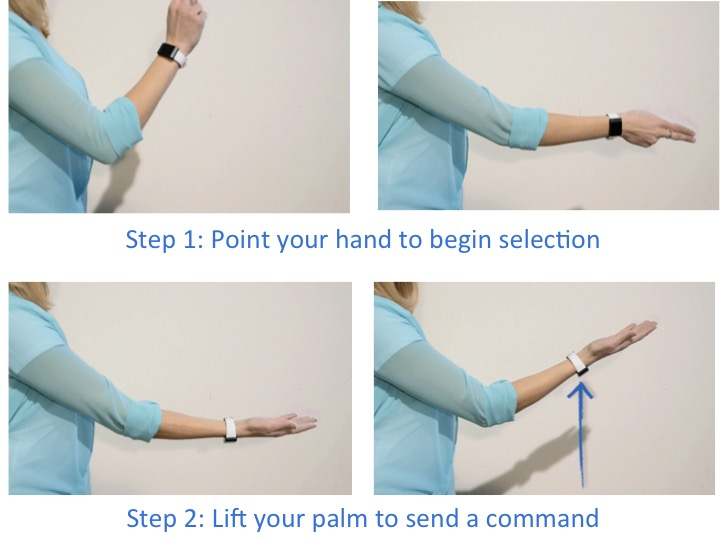
\includegraphics[width=0.65\textwidth]{images/reemo}
\caption{Using the Reemo wearable to control a smart device. Image from~\cite{prespecialisation}.}
\label{fig:introduction:gesture-control:reemo}
\end{figure}

In~\cite{caon2011context} a solution for recognizing context-aware motion gestures using multiple Kinects is presented. Users control devices by pointing at them and depending on the current state of the device and the position of the user, different actions are triggered.
The authors use two Kinects to position the user and recognize motion gestures in a living room, requiring a total of 6-8 Kinects in an apartment consisting of 3-4 rooms. The high number of  Kinects results in a high price for installing the system. Furthermore there may be privacy concerns when using Kinects, as the cameras can be utilized for malicious activity.

In contrast to the previous solutions, the solution presented in this report differs in the way, that controllable devices are not required to be within line of sight. Users are able to control all devices within the system from anywhere in their house.

The solution will utilize beacons for positioning users as opposed to Kinects as utilized in~\cite{caon2011context}. This lowers the entry barrier by decreasing the initial cost as well as the cost for scaling the system to more rooms.

By utilizing an accelerometer, a common component in wearables~\cite[pp. 3-4]{prespecialisation}, the user may not need to buy hardware specifically for recognizing gestures.

%%% Local Variables:
%%% mode: latex
%%% TeX-master: "../../master"
%%% End:
